\setcounter{chapter}{2}
\chapter{El modelo central de la economía geográfica}
\pagenumbering{arabic}
\section{Introducción}
\textbf{Hace mucho tiempo que Ohlin (1933) observó que los campos de la teoría del comercio por un lado y la economía regional y urbana por el otro tenían, en principio, los mismos objetivos de investigación. Ambas áreas de investigación quieren responder a las preguntas: ¿Quién produce qué, dónde y por qué?} A pesar de la observación de Ohlin, cada campo ha seguido su propio camino desde el siglo XIX. Ya se demostró que la teoría del comercio asume que los países son puntos adimensionales en el espacio. \textbf{Los teóricos del comercio están interesados principalmente en cómo interactúan la estructura del mercado, las técnicas de producción y el comportamiento del consumidor} (Neary, 2004). Los precios resultantes de los factores y las materias primas determinan el patrón de los flujos comerciales internacionales. La ubicación es, en el mejor de los casos, un factor exógeno y, por lo general, no juega un papel significativo. \textbf{La economía regional y urbana, por el contrario, toma la estructura del mercado y los precios como dados y trata de averiguar qué asignación de espacio es más eficiente}. El comportamiento subyacente de consumidores y productores, central en la teoría del comercio, es menos importante (Fujita y Thisse, 1996). Aunque ambas corrientes de la literatura producen ideas valiosas por derecho propio, \textbf{la teoría del comercio y la economía regional y urbana se combinan productivamente en la economía geográfica.}\\   

Analizaremos y explicaremos el modelo central de la economía geográfica, un pequeño modelo de equilibrio general desarrollado por Krugman (1991a, 1991b). Como veremos, \textbf{las ecuaciones de equilibrio de este modelo no son lineales. Esto significa que los pequeños cambios en los parámetros no siempre producir los mismos efectos; a veces los efectos son pequeños, a veces son grandes.} Traducido a la economía regional y urbana, esto significa, por ejemplo, que la decisión de ubicación de un solo productor podría no cambiar el patrón espacial de producción, pero podría tener efectos dramáticos o catastróficos (tomando prestado un término de la literatura del caos). , Consecuencias. Es posible que la decisión de ubicación de un solo productor desencadene un proceso de causalidad acumulativa y que el patrón espacial de producción cambie drásticamente. Además, el modelo tiene múltiples equilibrios, y esta característica es, como hemos explicado en el capítulo 2, una de las principales diferencias con la ciencia regional o la economía urbana. No se presupone qué la ubicación podría convertirse en el centro de producción, pero una vez que una ubicación obtiene una ventaja, el proceso de causalidad acumulativa comienza a funcionar. Lo que inicialmente son pequeñas diferencias entre ubicaciones pueden evolucionar con el tiempo en grandes diferencias en el equilibrio a largo plazo. Estas y otras características hacen que los modelos de economía geográfica sean analíticamente complicados.\\

\section{Un ejemplo de la economía geográfica}
Es posible construir un ejemplo simple para ilustrar algunos de los principales hallazgos del enfoque de economía geográfica. Supongamos que hay dos regiones (o países), Norte y Sur, y dos sectores de producción, manufactura y agricultura. La industria manufacturera produce variedades, es decir, productos diferenciados, bajo economías internas de escala. Por lo tanto, el costo por unidad de producción cae a medida que una empresa expande su nivel de producción. Como resultado, cada empresa produce solo una variedad. Una empresa puede residir en el Norte o en el Sur, es decir, una empresa tiene que decidir dónde producir. Esta decisión de ubicación diferencia esencialmente el ejemplo de la nueva teoría comercial.\\
\begin{center}
\begin{tabular}{lccc}
    &Ventas norte&Ventas sur& Ventas totales\\\\
    \hline\\
    Todas las empresas en el norte & 5+5=8 & 0+2=2 & 10\\
    Todas las empresas en el sur & 0+4=4 & 4+2=6 & 10\\
    $25\%$ de empresas en el norte, & 1+4=5 & 3+2=5 & 10\\
    $75\%$ de empresas en el sur. & & & \\\\
\end{tabular}
\end{center}

La demanda total de cada variedad de manufacturas en este ejemplo es exógena. Suponemos que cada empresa vende cuatro unidades a los trabajadores de la industria manufacturera y seis unidades a los agricultores. Por lo tanto, la demanda total de cada variedad es diez (6 + 4). La producción de la agricultura, y por lo tanto la demanda que genera, es específica de la ubicación. Su distribución espacial está dada exógenamente; suponemos que se venden cuatro unidades en el Norte y dos unidades en el Sur. La ubicación de los trabajadores en el sector manufacturero y, por tanto, las cuatro unidades que demandan en esa ubicación, no es exógena. El papel de los trabajadores inmóviles es importante, ya que aseguran que siempre haya una demanda positiva en ambas regiones. Finalmente, los costos de transporte entre el Norte y el Sur son 1 euro por unidad. Las empresas deciden su ubicación para minimizar los costos de transporte.\\
Ahora podemos determinar la decisión de ubicación de cada empresa. Primero, podemos calcular las ventas regionales de cada empresa, dada la ubicación de las otras empresas. En la tabla de arriba, se dan tres posibilidades (no exhaustivas): todas las empresas en el Norte, todas las empresas en el Sur y el 25 por ciento de todas las empresas en el Norte y el 75 por ciento de todas las empresas en el Sur. Las ventas en cada región son iguales a las ventas a los trabajadores en la manufactura más las ventas a los agricultores. Tomemos, por ejemplo, la última fila de la tabla.  La empresa vende cinco unidades en el Norte, a saber, cuatro a los agricultores ubicados en Norte más un ($ = 25\% · 4)$ unidad a los trabajadores de manufactura ubicados en Norte. De manera similar, la empresa vende cinco unidades en el Sur, es decir, dos unidades a los agricultores ubicados en el Sur más tres $( = 75\% · 4)$ unidades a los trabajadores de manufactura ubicados en el Sur.\\
En segundo lugar, usando la tabla podemos construir una tabla de decisión, calculando los costos de transporte en función de la decisión de ubicación de la empresa, dada la ubicación de las otras empresas. Suponga, por ejemplo, que todas las empresas están ubicadas en el norte. La tabla de abajo indica que los costos de transporte para una empresa ubicada en el Sur serán entonces 8 euros, es decir, 4 euros para las ventas a los agricultores del Norte y 4 euros para las ventas a todos los trabajadores de la industria manufacturera ubicada en el Norte (haciendo abstracción de las ventas a sus propios trabajadores). De manera similar, si la empresa se ubica en el norte, los costos de transporte serían solo 2 euros para las ventas a los agricultores del sur. Dado que los costos de transporte se minimizan al ubicarse en el Norte si todas las demás empresas están ubicadas en el Norte, la empresa decide ubicar también la producción en el Norte. Como muestra el cuadro  (segunda fila), una empresa se ubicará en el Sur si todas las demás empresas también se ubican allí, mientras que (última fila) a la empresa le es indiferente ubicarse en el Norte o en el Sur (ya que los costos de transporte son los mismos si la empresa se ubica en el Sur). En cualquier región si el 25 por ciento de las empresas están ubicadas en el Norte y el 75 por ciento en el Sur.

\begin{center}
    \begin{tabular}{lcc}
	& Ubicado en el Norte & Ubicado en el sur \\\\
	\hline\\
	Todas las empresas Norte & 0+\textbf{2}=2 (Agricultor Sur) & 4+4=8 (Trabajador/agricultor Norte)\\
	Todas las empresas Sur &4+2=6 (Trabajador/agricultor Sur)& 0+4=\textbf{4} (Agricultor Norte)\\
	$25\%$ de agricultores Norte, & 3+2=5 (trabajador/agricultor Sur) & 1+4=5 (Trabajador/agricultor Norte)\\
	$75\%$ de agricultores Sur & &  \\
	\hline\\
    \end{tabular}
    Costos de transporte
\end{center}
\vspace{.5cm}

En primer lugar, el concepto de causalidad acumulativa. Si, por alguna razón, una ubicación ha atraído a más empresas que la otra ubicación, una nueva empresa tiene un incentivo para ubicarse donde están las otras empresas. Tome la primera fila en la tabla de arriba. Si todas las empresas existentes están ubicadas en el norte, la nueva empresa también debería ubicarse allí si desea minimizar sus costos de transporte. De manera similar, para la segunda fila,  la empresa se ubicará en el sur.\\
En segundo lugar, la tabla  ilustra la existencia de equilibrios múltiples. La aglomeración de todas las empresas en el Norte o en el Sur es un equilibrio. Sin embargo, no podemos determinar de antemano dónde ocurrirá la aglomeración. Esto depende críticamente de las condiciones iniciales, es decir, las decisiones previas de ubicación de otras empresas.\\
Tercero, un equilibrio puede ser estable o inestable. Las entradas en negrita en la tabla  son ambos equilibrios estables si una sola empresa decide mudarse, esto decisión no influiría en las decisiones de ubicación de las otras empresas. La última fila  describe un equilibrio inestable. Si una sola empresa decide trasladarse, la nueva ubicación se volverá inmediatamente más atractiva para todas las demás empresas. Esto desencadenará un efecto bola de nieve: todas las empresas seguirán al pionero. En este ejemplo, solo la aglomeración es un equilibrio estable.\\
En cuarto lugar, observamos que un equilibrio estable puede no ser óptimo. Si todas las empresas están ubicadas en el norte, los costos de transporte son solo 2 euros. Si todas las empresas están ubicadas en el sur, los costos de transporte son 4 euros.  Por lo tanto, los costos de transporte para la economía en su conjunto se minimizan si todas las empresas se aglomeran en el Norte, mientras que la aglomeración en el Sur sigue siendo un equilibrio estable.\\
En quinto lugar, el ejemplo ilustra la interacción de la aglomeración y los flujos comerciales. Con la aglomeración completa, es decir, todas las manufacturas se producen en una sola región, el comercio entre regiones será de tipo interindustrial (alimentos para manufacturas). De hecho, este equilibrio también refleja el llamado efecto del mercado doméstico; la combinación de economías de escala y costos de transporte es responsable del agrupamiento de toda la actividad libre en un solo lugar. Debido a esta combinación, los costos de transporte pueden minimizarse. La gran región termina con un gran mercado para la fabricación de bienes, que pueden venderse sin incurrir en costos de transporte. La consecuencia es que esta región se convierte en exportadora de productos manufacturados; Las grandes regiones tienden a convertirse en exportadoras de aquellos bienes para los que tienen un gran mercado local, de ahí el término efecto del mercado interno. Si la industria manufacturera está ubicada en ambas regiones, como se describe en las últimas filas de los cuadros, el comercio también será del tipo intraindustrial. Además de intercambiar bienes manufacturados por productos agrícolas, se intercambiarán diferentes variedades de productos manufacturados diferenciados entre ambas regiones.\\
El ejemplo es útil, ya que ilustra algunos aspectos importantes de la economía geográfica. Sin embargo, un ejemplo es solo un ejemplo y no es un sustituto de un modelo bien especificado. ¿Qué falta en el ejemplo?\\
\begin{itemize}
    \item \textbf{En primer lugar, falta la interacción entre los costos de transporte, el comportamiento de fijación de precios y la elección de la ubicación.} Simplemente suponemos que la demanda que enfrenta cada empresa está dada y es independiente del comportamiento de fijación de precios y los costos de transporte. De hecho, los precios faltan por completo en el ejemplo. No hay análisis de la estructura del mercado. En realidad, los precios, los salarios y los costos de transporte determinarán el poder adquisitivo de los consumidores. Uno podría suponer que esta interacción impulsa las decisiones de ubicación de consumidores y productores. Las siguientes secciones muestran que este es, de hecho, el caso.
    \item Además, es un modelo de equilibrio parcial, en el sentido de que las empresas no se preocupan por la mano de obra necesaria; donde sea que decidan ubicarse, \textbf{la disponibilidad de mano de obra no es el problema.} Resultará que los supuestos con respecto al funcionamiento del mercado laboral son importantes. El lector también puede notar la similitud del ejemplo y el nuevo modelo de comercio de Krugman (1980) discutido en el capítulo 2. En ambos modelos, las economías de escala y los costos de transporte son fuerzas importantes. La diferencia más importante es que, en nuestro ejemplo, las empresas pueden ubicarse en cualquier región. En consecuencia, el ejemplo da lugar a aglomeraciones y equilibrios múltiples.
\end{itemize}

\section{La estructura del modelo.}

Esta sección ofrece una descripción general no técnica de la estructura general del modelo central de la economía geográfica. Los aspectos básicos del modelo central se exponen en Dixit y Stiglitz (1977) y Krugman (1979, 1980). Estos trabajos estimularon una gran cantidad de trabajo sobre competencia monopolística y teoría del comercio internacional. Krugman (1991a, 1991b) extiende este último al permitir la movilidad de factores interregionales, y esto se ha convertido en el modelo central de la economía geográfica. Esta estructura se ilustra en la figura de abajo. \\
El modelo central identifica dos regiones, etiquetadas como 1 y 2. Hay dos sectores en la economía, el sector manufacturero y el sector alimentario. Los consumidores en ambas regiones consisten en trabajadores agrícolas y trabajadores de manufactura. Los trabajadores agrícolas obtienen sus ingresos trabajando en las granjas de su región. El flujo de ingresos de los trabajadores agrícolas es parte de una transferencia bilateral: obtienen un ingreso a cambio de su oferta de mano de obra. Todas esas transferencias bilaterales se indican con flechas de dos puntas. La flecha de punta sólida indica la dirección de los flujos de dinero o ingresos, es decir, indica la dirección de los ingresos y los gastos. Lo que representa el flujo se indica a lo largo de la línea que conecta los puntos de flecha. La flecha de punta abierta indica la dirección de los flujos de bienes o servicios. Estos se indican entre paréntesis a lo largo de la línea que conecta los puntos de flecha. \textbf{Los agricultores de la región 1 producen alimentos bajo rendimientos constantes a escala y competencia perfecta}. Venden este alimento a los consumidores, ya sea en la región 1 o en la región 2. Por supuesto, no hay costos de transporte para los alimentos.\\

\begin{center}
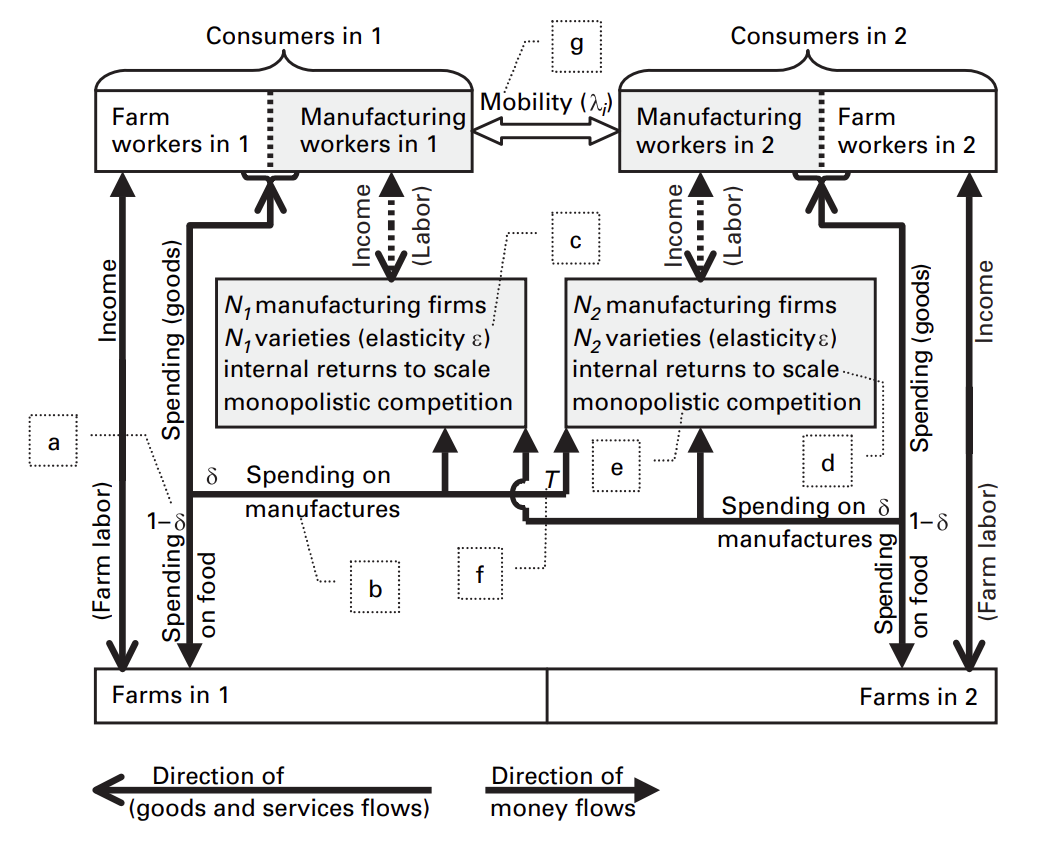
\includegraphics[scale=.3]{./imagen/diag.png}
\end{center}

El sector manufacturero consta de empresas $N1$ en la región 1 y empresas $N2$ en la región 2. Cada empresa manufacturera produce un producto diferenciado, es decir, produce una variedad única de manufacturas. \textbf{Utiliza solo mano de obra en el proceso de producción, que se caracteriza por economías internas de escala. Esto implica que las empresas tienen poder de monopolio, que utilizan para determinar el precio de su producto. Además, los costos de transporte están involucrados en la venta de un bien manufacturado en otra región. Estos costos no surgen si el bien manufacturado se vende en la región en la que se produce. Como resultado de los costos de transporte, las empresas exportadoras cobrarán un precio más alto en la región extranjera que en la región de origen.} Los trabajadores manufactureros obtienen sus ingresos (la tasa salarial manufacturera) al suministrar mano de obra a las empresas del sector manufacturero ubicadas en la región de origen.\\
Los consumidores gastan sus ingresos tanto en alimentos como en manufacturas. Dado que los alimentos son un bien homogéneo, no les importa si se producen en la región 1 o en la región 2. Como los alimentos no tienen costos de transporte, tienen el mismo precio en ambas regiones (lo que implica que los agricultores ganan el mismo salario en ambas regiones). El gasto de los consumidores en manufacturas debe distribuirse entre las muchas variedades producidas en las regiones 1 y 2. \textbf{En igualdad de condiciones, consumir variedades importadas es más costoso que consumir variedades nacionales, como resultado de los costos de transporte de los productos manufacturados.} Sin embargo, dado que las variedades son productos diferenciados y los consumidores tienen gusto por la variedad, siempre consumirán algunas unidades de todas las variedades producidas, ya sea en el país o en el extranjero.\\
Se imponen algunas observaciones finales sobre la figura. Primero, la figura menciona los parámetros más importantes que se usarán en el resto de este libro, a saber, $\epsilon, \delta, \lambda_i$ y $T$. En este punto no es importante saber cuáles son estos parámetros. Ellos, y otros, serán discutidos en el resto de este capítulo. En segundo lugar, la figura  muestra siete rótulos, etiquetados de la $a$ la $g$. Estas anotaciones se refieren a detalles de construcción importantes del modelo central. Se utilizan como referencia y recordatorio en la sección 3.4 sobre la estructura de demanda del modelo (rótulos a, b y c), en la sección 3.5 sobre la estructura de oferta del modelo (rótulos d y e), en la sección 3.6 sobre el papel de los costos de transporte (llamada f) y en la sección 3.9 sobre la dinámica del modelo (llamada g). En tercer lugar, y lo más importante, hay cuadros sombreados en la figura. Estos llaman la atención sobre la característica distintiva de la economía geográfica: la movilidad de los factores de producción. El modelo central aplica la movilidad solo al sector manufacturero; los trabajadores de fabricación pueden trasladarse de la región 1 a la región 2, o viceversa. \textbf{La reubicación de empresas manufactureras de una región a otra es la otra cara de la misma moneda, ya que una expansión de la mano de obra manufacturera en una región implica una expansión de la producción en el sector manufacturero.} Es importante señalar que, en principio, las casillas sombreadas pueden desaparecer en una región, por ejemplo, si todos los trabajadores de fabricación (y, por lo tanto, todo el sector manufacturero) se trasladan a la región 2. Las casillas no sombreadas, etiquetadas como trabajadores agrícolas y granjas, no pueden desaparecer de una región. Los agricultores necesitan la tierra para el cultivo y, por lo tanto, no son móviles. La región, por lo tanto, siempre puede gastar los ingresos generados por este sector. La distinción entre actividad móvil y actividad inmóvil es importante. Para facilitar la referencia, hemos etiquetado estos sectores como manufacturas y alimentos, respectivamente. Obviamente, el sector inmobiliario también podría producir mineral de hierro o papel, o producir un servicio no transable (vivienda), etc.\\

\paragraph{Terminología}

\textbf{Aglomeración y dispersión.} Estamos interesados en explicar y describir varias formas de agrupación de actividad (económica), a las que nos referimos como aglomeración. Usamos el término difusión para referirnos a lo contrario de aglomeración. Otros términos utilizados en la literatura, como centrípeto, centrífugo, convergente y divergente, no se utilizarán en este libro porque pueden ser confusos. Por ejemplo, la palabra convergente puede indicar que todas las industrias convergen, es decir, tienden a ubicarse en una región, o que todas las regiones convergen, es decir, todas las industrias están distribuidas entre regiones.\\
\textbf{Numerario}. Los agentes económicos en los modelos de equilibrio general de la economía geográfica no sufren de ilusión monetaria, es decir, sus decisiones se basan en precios relativos y no dependen del nivel absoluto de precios. Esto nos permite establecer el precio de uno de los bienes del modelo igual a uno, y expresar todos los demás precios del modelo en relación con el precio del bien numerario. El resto del libro elige la comida como bien numerario, de modo que el precio de la comida siempre es igual a uno.\\
\textbf{Salarios y salarios reales.} El enfoque central de modelado de equilibrio general utilizado en este libro elige un bien numérico para precisar los precios relativos. Los salarios en diferentes regiones expresados en el numerario deben denominarse salarios numerarios. Aunque es mejor que el término de uso frecuente salarios nominales (ya que el sector monetario no se modela explícitamente), sigue siendo un término engorroso. Por lo tanto, usamos el término más corto salario cada vez que nos referimos a salario numérico, y usamos explícitamente el término salario real cuando los salarios numéricos se corrigen por el nivel de precios para determinar el poder adquisitivo.

\section{Demanda}

\subsection{Gasto en alimentos y manufacturas (a)}
\textbf{Como se explicó en la sección 3.3, la economía tiene dos sectores de bienes, manufacturas, $M$, y alimentos, $F$. Aunque las manufacturas consisten en muchas variedades diferentes, podemos definir un índice de precios exacto para representarlas como un grupo. A este índice de precios de manufacturas lo llamamos I.} Si un consumidor obtiene un ingreso Y (por trabajar en el sector alimentario o en el sector manufacturero), tiene que decidir cuánto de este ingreso se gasta en alimentos y cuánto en manufacturas. La solución a este problema depende de las preferencias del consumidor, que se suponen de la especificación Cobb-Douglas dada en la ecuación (3.1) para todos los consumidores, en la que $F$ representa el consumo de alimentos y $M$ representa el consumo de manufacturas:
\begin{equation}
    U=F^{1-\delta} M^\delta;\qquad 0<\delta<1
\end{equation}

Obviamente, cualquier ingreso gastado en alimentos no puede gastarse simultáneamente en manufacturas, es decir, el consumidor debe satisfacer la restricción presupuestaria en la ecuación (3.2):

\begin{equation}
    F+I \cdot M=Y
\end{equation}

\textbf{Nótese la ausencia del precio de los alimentos en esta ecuación. Esto es el resultado de elegir los alimentos como numerario, lo que implica que el ingreso $Y$ se mide en términos de alimentos.} Por lo tanto, solo el índice de precios de las manufacturas $I$ aparece en la ecuación (3.2). Para decidir sobre la asignación óptima de ingresos sobre la compra de alimentos y manufacturas, el consumidor ahora tiene que resolver un problema de optimización simple, a saber, maximizar la utilidad como se indica en la ecuación (3.1), sujeto a la restricción presupuestaria de la ecuación (3.2). La solución a este problema se da en la ecuación (3.3), y se deriva de la nota de más abajo.

\begin{equation}
    F=(1-\delta)Y;\qquad IM=\delta Y
\end{equation}

Como muestra la ecuación (3.3), es óptimo que el consumidor gaste una fracción $(1 -\delta)$ de su ingreso en alimentos y una fracción, $\delta$, de su ingreso en manufacturas. Esto explica la leyenda a en la figura de arriba. De ahora en adelante nos referiremos al parámetro d dado en la ecuación (3.1) como la fracción del ingreso gastado en manufacturas.

\begin{nota}[Derivación de la ecuación]
    Para maximizar la ecuación (3.1) sujeta a la restricción presupuestaria (3.2), definimos el Lagrangiano C, usando el multiplicador j:
    $$\Gamma F^{1-\delta}M^\delta + k[Y-(F+IM)]$$
    La diferenciación de C con respecto a F y M da las condiciones de primer orden
    $$(1-\delta)F^{-\delta}M^\delta = k\; \qquad \delta F^{1-\delta}M^{\delta-1}=kI$$
    Tomando la relación de las condiciones de primer orden se obtiene
    $$\dfrac{\delta F^{1-\delta} M^{\delta - 1}}{(1-\delta)F^{-\delta}M^\delta};\qquad IM = \dfrac{\delta}{1-\delta}F$$
    Sustituyendo este último en la ecuación presupuestaria (3.2) se obtiene
    $$Y=F+IM = F+\dfrac{\delta}{1-\delta}F;\qquad F=(1-\delta)Y$$
\end{nota}

\subsection{Gasto en la fabricación de manufacturas (b)}
Ahora que hemos determinado en la subsección 3.4.1 la parte $\delta$ del ingreso que se gasta en bienes manufacturados, todavía tenemos que decidir cómo se distribuye este gasto entre las diferentes variedades de manufacturas. En esencia, este es un problema similar al de la subsección 3.4.1, es decir, tenemos que asignar de manera óptima el gasto entre el consumo de una cantidad de bienes que se pueden consumir. Este problema sólo puede resolverse si especificamos cómo las preferencias por el consumo agregado de manufacturas $M$ dependen del consumo de variedades particulares de manufacturas. A este respecto, \textbf{el modelo central de la economía geográfica aplica fructíferamente un modelo de competencia monopolística desarrollado en la literatura sobre organización industrial por Dixit y Stiglitz }. Sea $c_i$ el nivel de consumo de una determinada variedad $i$ de manufacturas, y sea $N$ el número total de variedades disponibles. El enfoque de Dixit-Stiglitz utiliza una función de elasticidad de sustitución constante (CES) para construir el consumo agregado de manufacturas M en función del consumo $c_i$ de las $N$ variedades:
\begin{equation}
    M=\left(\sum_{i=1}^N c^{\rho}_i \right)^{1/\rho}
\end{equation}

Tenga en cuenta que el consumo de todas las variedades entra en la ecuación (3.4) simétricamente. Esto simplifica enormemente el análisis en el resto del capítulo. El parámetro $\rho$, discutido más adelante, representa el efecto de gustos por la variedad de los consumidores. Si $\rho = 1$, la ecuación (3.4) se simplifica a $M = \sum_i ci$ y la variedad como tal no importa para la utilidad (tener $100$ unidades de una variedad da la misma utilidad que una unidad de $100$ variedades). Los productos son entonces sustitutos perfectos (una unidad menos de una variedad puede compensarse exactamente con una unidad más de otra variedad). Por lo tanto, necesitamos $\rho < 1$ para asegurar que las variedades de productos sean sustitutos imperfectos. Además, necesitamos $\rho > 0$ para garantizar que las variedades individuales sean sustitutos (y no complementos) entre sí, lo que permite un comportamiento de fijación de precios basado en el poder de monopolio.\\
Vale la pena detenerse un poco más en la especificación de (3.4). Suponga que todos los $c_i$ se consumen en cantidades iguales, es decir, $c_i= c$ para todos los $i$. Entonces podemos reescribir la ecuación (3.4) como

$$M=\left(\sum_{i=1}^N c^\rho\right)^{1/\rho} = (Nc^\rho)^{1/\rho} = N^{1/\rho} c = N^{(1/\rho)}[Nc] \qquad \hspace{2cm} (3.4^{'})$$

Como $0 < \rho < 1$, el término $(1/\rho)- 1$ es mayor que cero. Entonces, a partir de $(3.4^{'})$ queda inmediatamente claro que tener $100$ unidades de una variedad $(Nc = C, N = 1)$ le da al consumidor menos utilidad que una unidad de $100$ variedades $(Nc = C, N = 100)$. En muchos modelos, incluidos muchos nuevos modelos de crecimiento y modelos de economía geográfica, el término $N_c$ en la ecuación $(3.4^{'})$ corresponde a un reclamo sobre recursos reales, porque $Nc$ tiene que ser producido en primer lugar, mientras que el número de variedades disponibles $N$ representa una externalidad o la extensión del mercado. El término $N(1/q)^{-1}$ representa una bonificación para grandes mercados, de ahí el término efecto de gustos por la variedad. En este sentido, un aumento en la extensión del mercado, que aumenta el número de variedades $N$ entre las que el consumidor puede elegir, aumenta más que proporcionalmente la utilidad.\\
Después de nuestra breve digresión sobre el efecto del amor por la variedad, es hora de volver al problema que nos ocupa: ¿cómo distribuye el consumidor el gasto en manufacturas entre las diversas variedades? Sea $p_i$ el precio de la variedad $i$ para $i = 1, . . . , N$. Naturalmente, los fondos $p_ic_i$ gastados en la variedad $i$ no pueden gastarse simultáneamente en la variedad $j$, como se indica en la restricción presupuestaria para manufacturas en la ecuación (3.5): 
\begin{equation}
    \sum_{i=1}^N p_i c_i = \delta Y
\end{equation}

Para derivar la demanda de un consumidor, ahora debemos resolver un problema de optimización algo más complicado, a saber, la maximización de la utilidad derivada del consumo de manufacturas dada en la ecuación (3.4), sujeta a la restricción presupuestaria de la ecuación (3.5). La solución a este problema se da en las ecuaciones (3.6) y (3.7), y se deriva de la nota técnica 3.2

\begin{equation}
    c_j = p_j^{-\epsilon} \left[I^{\epsilon-1}\delta Y\right], \qquad \mbox{donde}\; I \equiv \left['\sum_{i=1}^N p_i^{1-\epsilon}\right]^{1/(1-\epsilon)} \quad \mbox{para}\; j=1,\ldots,N
\end{equation}

\begin{equation}
    M=\delta Y / I, \quad \mbox{y}\quad \epsilon \equiv \dfrac{1}{1-\rho}
\end{equation}
En este punto, lo importante es enfatizar que la ecuación (3.6) da la curva de demanda. Concluimos esta subsección simplemente señalando que hemos derivado la demanda para cada variedad de manufacturas, lo que explica la llamada b en la figura

\paragraph{Competencia monopolística Dixit-Stiglitz.}
A menudo se ha dicho que solo hay una forma de que la competencia sea perfecta, pero muchas formas de ser imperfecta. En consecuencia, existen muchos modelos en competencia para describir la competencia imperfecta, investigando muchos casos y supuestos diferentes con respecto al comportamiento del mercado, el tipo de bien, la interacción estratégica entre empresas, las preferencias de los consumidores, etc. Ese también fue el caso de la competencia monopolística (ver , por ejemplo, Tirole, 1988), hasta que Dixit y Stiglitz publicaron en 1977 un artículo titulado “Competencia monopolística y la diversidad óptima de productos”, en The American Economic Review, que revolucionaría la construcción de modelos en al menos cuatro campos de la economía: el comercio teoría, organización industrial, teoría del crecimiento y economía geográfica.\\
El gran paso adelante fue hacer algunas suposiciones heroicas sobre la simetría de las nuevas variedades y la forma estructural, lo que permitió una forma elegante y consistente de modelar la producción a nivel de empresa, beneficiándose de las economías de escala internas junto con una estructura de mercado de competencia monopolística, sin caer en una taxonomía de modelos de oligopolio. Estos factores son los responsables de la actual popularidad del modelo Dixit-Stiglitz. En todos los campos que ahora usan intensamente la formulación de Dixit-Stiglitz, los investigadores eran conscientes de que la competencia imperfecta era relevante como una característica esencial de muchos fenómenos observados empíricamente. Esto significó que el modelo fue inmediatamente aceptado como el nuevo estándar para modelar la competencia monopolística; su desarrollo fue ciertamente muy oportuno. En la teoría del comercio internacional, la introducción del modelo de competencia monopolística permitió a los economistas internacionales explicar y comprender el comercio intraindustrial, que hasta entonces había sido observado empíricamente pero nunca explicado satisfactoriamente (Krugman, 1979, 1980). En la organización industrial, ayudó a deshacerse de muchos supuestos ad hoc, que dificultaron el desarrollo de muchos modelos de organización industrial (Tirole, 1988). El modelo Dixit-Stiglitz también se utilizó para explorar el papel de los bienes intermedios diferenciados en los modelos de comercio internacional. Esta reformulación del modelo estándar de Dixit-Stiglitz juega un papel importante en el vínculo entre el comercio internacional y el crecimiento económico (ver, por ejemplo, Grossman y Helpman, 1991). El modelo también resulta muy útil para explicar la decisión de exportar IED si las empresas son heterogéneas (véanse Melitz, 2003 y Helpman, Melitz y Yeaple, 2004). Finalmente, el modelo se usa intensamente en economía geográfica, el tema de este libro.

\subsection{\boldmath Efectos de la demanda: renta, precio, elasticidad $\epsilon$ (c) y el índice de precios I}
La demanda de la variedad 1, por ejemplo, está dada por $c_1 = p_1^{-\epsilon} \left[I^{\epsilon-1} \delta Y\right]$ (ecuación 3.6). Esta demanda parece estar influenciada por cuatro cosas, a saber (i) el ingreso $\delta Y$ gastado en manufacturas en general, (ii) el precio $p_1$ del bien $1$, (iii) algún parámetro $\epsilon$, y (iv) el índice de precios $I$. \\
El punto (i) es sencillo. Cuanto más gasta el consumidor en manufacturas en general, más gasta en la variedad $1$. De hecho, esta relación es equiproporcional: en igualdad de condiciones, un aumento del $10$ por ciento en el gasto en manufacturas da como resultado un aumento del $10$ por ciento en la demanda para todas las variedades de manufacturas.\\
El punto (ii) también es sencillo, pero muy importante. Es sencillo en el sentido de que obviamente esperamos que la demanda de la variedad $1$ sea una función del precio cobrado por la empresa que produce la variedad $1$. Es muy importante en vista de cómo la demanda de la variedad $1$ depende del precio $p_1$. Tenga en cuenta que la última parte de la ecuación (3.6) está escrita entre corchetes. Depende del índice de precios de las manufacturas $I$ y del ingreso $\delta Y$ gastado por los consumidores en manufacturas en general. Ambas son entidades macroeconómicas que la empresa que produce la variedad $1$ tomará como dadas, es decir, asumirá que no tiene control sobre estas variables. En ese caso, podemos simplificar la demanda de la variedad $1$, definiendo $constante_1 \equiv [I^{\epsilon-1} \delta Y]$ como $c_1 = constante_1 p_1^{-\epsilon}$ . Esto, a su vez, implica que la elasticidad precio de la demanda de la variedad $1$ es constante e igual al parámetro $\epsilon > 1$ (es decir, $-\left(\partial c_1/\partial p_1\right)\left(p_1/c_1\right)=\epsilon$. Esta simple elasticidad precio de la demanda es la principal ventaja del enfoque Dixit-Stiglitz, ya que simplifica enormemente el comportamiento de fijación de precios de las empresas monopolísticamente competitivas. La demanda de una variedad de manufacturas en función de su propio precio para diferentes valores de $\epsilon$. Tenga en cuenta que la demanda de una variedad cae mucho más rápidamente como resultado de un pequeño aumento de precio, digamos de $1$ a $1.5$, si la elasticidad precio de la demanda es alta.\\
El punto (iii) queda claro después de la discusión en el punto (ii). Hemos definido el parámetro $\epsilon$ no solo para simplificar la notación de la ecuación (3.6) tanto como sea posible, sino también porque es un parámetro económico importante, ya que mide la elasticidad precio de la demanda de una variedad de bienes manufacturados. Además, como se discutió en la subsección anterior, este parámetro mide la elasticidad de sustitución entre dos variedades diferentes, que es decir, cuán difícil es sustituir una variedad de manufacturas por otra variedad de manufacturas. Evidentemente, la elasticidad precio de la demanda y la elasticidad de sustitución están relacionadas en el enfoque de Dixit-Stiglitz, un punto que ha sido criticado en la literatura.  Sea como fuere, nuestras explicaciones intuitivas de algunos fenómenos en el resto de este libro a veces se basarán en la interpretación de la elasticidad precio de la demanda de $\epsilon$, y a veces en la interpretación de la elasticidad de sustitución, usando lo que creemos que es más fácil para el problema en cuestión.\\
Se impone una observación final sobre el parámetro $\epsilon$. Se definió usando el parámetro $\rho$ en la ecuación de preferencia por variedades de manufactura (3.4) como $\epsilon \equiv 1/(1-\rho)$. Estos son los dos únicos parámetros para los que haremos esto, refiriéndose a $\epsilon$ como la elasticidad de sustitución y a $\rho$ como el parámetro de sustitución. Es útil tener presente su relación.\\
Finalmente, el punto (iv) indica que la demanda de la variedad $1$ depende del índice de precios $I$. Si el índice de precios $I$ aumenta, lo que implica que en promedio los precios de las variedades de fabricación que compiten con la variedad $1$ están aumentando, entonces la demanda de la variedad $1$ es creciente (recuerde que $\epsilon-1>0$). Las variedades son, por lo tanto, sustitutos económicos entre sí (si el precio de una variedad en particular aumenta, su propia demanda cae y la demanda de todas las demás variedades aumenta).\\
Tenga en cuenta que, aunque pueda parecer un poco engorroso a primera vista, el índice de precios $I$ en la ecuación (3.6) se define de manera análoga a la función en la ecuación (3.4) que especifica la preferencia por las variedades, con $1 – \epsilon$ en (3.6) jugando el papel principal de $\rho$ en (3.4). De hecho, si usamos esta información para calcular la elasticidad de sustitución de los precios en la ecuación (3.6) obtenemos $1/[1 - (1 - \epsilon)] = 1/\epsilon$, la inversa de la elasticidad de sustitución de las variedades. Esto no es una coincidencia, ya que indica que si la elasticidad de sustitución de variedades es alta, un pequeño cambio de precio puede tener grandes efectos, y viceversa si es pequeño. Sin embargo, lo más importante es tener en cuenta que la definición del índice de precios $I$ implica que $M = delta Y/I$ (ecuación (3.7)). El índice de precios $I$ da así una representación exacta de la utilidad derivada del consumo de manufacturas; esta utilidad aumenta si, y solo si, el gasto en manufacturas aumenta más rápidamente que el índice de precios $I$. También tenga en cuenta que se requiere $IM = \delta Y$ para justificar nuestras acciones en la subsección 3.4.1, donde usamos el índice de precios $I$ para derivar la división de los ingresos sobre el consumo de alimentos y trabajo consumo. De lo contrario, nuestros cálculos allí no habrían sido consistentes.\\
Con frecuencia usamos el índice de precios $I$ para derivar los salarios reales en el modelo. Por lo tanto, vale la pena echar un vistazo más de cerca a la definición de índices de precios basados en el consumo. Puede hacerse la pregunta ¿Cuál es la cantidad mínima de gasto requerida para comprar una unidad de utilidad? Sea $I$ este gasto mínimo en manufacturas, tal que $M =1$. Entonces llamamos índice de precios exacto o basado en el consumo. De esta definición se sigue directamente de las ecuaciones (3.5) y (3.7) que $I$ es de hecho tal índice. Es obvio que un aumento en el número de variedades disminuye $I$. Ya hemos explicado que un aumento en el número de variedades aumenta más que proporcionalmente la subutilidad de las manufacturas. Este efecto tiene una imagen especular en el índice de precios $I$; \textbf{\boldmath más variedades reducen $I$, porque se requiere menos gasto para $M = 1$}. Además, el término I nos permitió escribir las ecuaciones de demanda de manera más eficiente como $c_j =  p_j^{-\epsilon} [I^{\epsilon-1} \delta Y]$.\\
Para concluir nuestra discusión sobre la estructura de demanda del modelo central, debemos hacer dos comentarios. El primero es relativamente corto. Podríamos usar el mismo procedimiento aplicado en la subsección 3.4.2 para derivar el índice de precios exacto para la asignación entre variedades para derivar dicho índice de precios para el problema de la subsección 3.4.1, asignación de ingresos entre alimentos y manufacturas. Como el lector querrá comprobar, el resultado sería $1^{1-\delta}I^{delta}=I^{\delta}$ , en el que el 1 de la izquierda representa el precio de los alimentos, el cual se iguala a uno por ser el numerario. Por lo tanto, la utilidad del consumidor aumenta si, y solo si, $Y/I^{\delta}$ aumenta, es decir, si el nivel de ingresos aumenta más rápidamente que el índice de precios exacto $I^{\delta}$ . Por lo tanto, podemos definir el ingreso real y como una representación exacta de las preferencias de un consumidor;  (ecuación (3.8)). De manera similar, si la tasa salarial es $W$, podemos definir el salario real $w$ también utilizando el índice de precios exacto (ecuación (3.8)). Además, si un consumidor individual sólo tiene renta salarial, es decir, si $Y = W$, entonces la renta real individual y es equivalente al salario real $w$.\\
    \begin{equation}
	ingreso\; real: \; y=YI^{-\delta};\qquad salario\; real: \; w=WI^{-\delta}
    \end{equation}

    La segunda observación se refiere al punto (ii) anterior, en el que argumentamos que la (propia) elasticidad precio de la demanda del productor de la variedad $1$ es igual a $\epsilon$. Recuerde la especificación de la función de demanda: $c_1 = p_1^{-\epsilon}[I^{\epsilon-1} \delta Y]$. Argumentamos que el término entre corchetes es tratado como una constante por el productor porque se trata de entidades macroeconómicas. Si bien esto es cierto, se pasa por alto un pequeño detalle: uno de los términos en la especificación del índice de precios de las manufacturas $I$ es el precio $p_1$. Por lo tanto, un productor verdaderamente racional también tendría en cuenta este minúsculo efecto sobre el índice de precios agregado.\\
Por esa razón, a menudo se supone que la cantidad de variedades $N$ producidas es grande, es decir, si nuestro productor es una de las $80 000$ empresas, podemos ignorar este efecto con seguridad. Donde representamos la curva de demanda a la que se enfrenta el productor de una variedad si asume que no puede influir en el índice de precios de las manufacturas, y la demanda real teniendo en cuenta este efecto sobre el índice de precios. Claramente, la suposición es una mala aproximación si solo hay dos empresas, pero nadie sugiere que se deba usar la competencia monopolística en un duopolio. Si hay veinte empresas la aproximación ya es mucho mejor, si hay $200$ empresas la desviación es prácticamente indetectable, mientras que es inobservable si hay $2000$ empresas. Esto sugiere que podemos ignorar con seguridad este detalle para un número razonablemente grande de variedades.


\section{Oferta}

\subsection{Estructura de producción (d)}
Comenzamos el análisis del lado de la oferta del modelo central con una descripción de la estructura de producción de alimentos y manufacturas. \textbf{La producción de alimentos se caracteriza por rendimientos constantes a escala, y los alimentos se producen en condiciones de competencia perfecta.} Se supone que los trabajadores de esta industria están inmóviles. El sector alimentario es, por lo tanto, el candidato natural para ser utilizado como numerario. Dada la fuerza laboral total $L$, se supone que una fracción $(1-\lambda)$ trabaja en el sector alimentario. Por lo tanto, la fuerza de trabajo en la industria manufacturera es $\lambda L$. La producción en el sector alimentario, $F$, es igual, por elección de unidades, al empleo alimentario:

\begin{equation}
    F=(1-\lambda)L;\qquad 0<\lambda<1
\end{equation}

Dado que a los trabajadores agrícolas se les paga el valor del producto marginal, esta elección de unidades implica que el salario de los trabajadores agrícolas es uno, porque la comida es el numerario.\\
\textbf{La producción en el sector manufacturero se caracteriza por economías de escala internas, lo que significa que existe una competencia imperfecta en este sector}. Las variedades en la industria manufacturera son simétricos y se producen con la misma tecnología. Tenga en cuenta que incluso en este punto ya hemos introducido un elemento de ubicación. \textbf{Las economías de escala internas significan que cada variedad es producida por una sola empresa}; la empresa con las mayores ventas siempre puede superar a un competidor potencial. Una vez que hayamos introducido más ubicaciones, cada empresa tiene que decidir dónde producir. Las economías de escala se modelizan de la forma más sencilla posible:

\begin{equation}
    l_i = a + \beta x_i
\end{equation}

donde $l_i$ es la cantidad de trabajo necesaria para producir $x_i$ de la variedad $i$. Los coeficientes $a$ y $\beta$ describen los requisitos de insumos de mano de obra fijos y marginales, respectivamente. El insumo de trabajo fijo $a$ en (3.10) asegura que a medida que la producción se expande, se necesita menos trabajo para producir una unidad de $x_i$, lo que significa que hay economías de escala internas. 

\subsection{Fijación de precios y beneficios cero (e)}
\textbf{Cada empresa manufacturera produce una variedad única bajo rendimientos internos a escala. Esto implica que la empresa tiene poder de monopolio, que utilizará para maximizar sus beneficios. Por lo tanto, tenemos que determinar la fijación de precios comportamiento de cada empresa.} El modelo de competencia monopolística de Dixit-Stiglitz hace dos supuestos a este respecto. En primer lugar, se supone que cada empresa toma como dado el comportamiento de fijación de precios de otras empresas; es decir, si la empresa $1$ cambia su precio, asumirá que los precios de las otras $N–1$ variedades seguirán siendo los mismos. En segundo lugar, se supone que la empresa ignora el efecto de cambiar su propio precio sobre el índice de precios $I$ de las manufacturas. Ambos supuestos parecen razonables si el número de variedades $N$ es grande. Para facilitar la notación, eliminamos el subíndice de la empresa en esta sección. Tenga en cuenta que una empresa que produce $x$ unidades de producción usando la función de producción en la ecuación (3.10) obtendrá ganancias $\pi$ dadas en la ecuación (3.11) si la tasa de salario que tiene que pagar es $W$.

\begin{equation}
    \pi = px-W(a+\beta x)
\end{equation}

Naturalmente, la empresa tendrá que vender las unidades de producción $x$ que está produciendo, es decir, estas ventas deben ser consistentes con la demanda de una variedad de manufacturas derivada. Aunque esta demanda se derivó para un consumidor arbitrario, la característica más importante de la demanda de una variedad, a saber, la elasticidad precio constante de la demanda $\epsilon$, también se cumple cuando combinamos la demanda de muchos consumidores con la misma estructura de preferencias. Si la demanda $x$ de una variedad tiene una elasticidad precio constante de la demanda $\epsilon$, la maximización de los beneficios dada en la ecuación (3.11) conduce a una regla de fijación de precios óptima muy simple, conocida como precio de sobreprecio, como se indica en la ecuación (3.12) y se deriva en la nota técnica:

\begin{equation}
    p(1-1/\epsilon)=\beta W \quad (o\; p=\beta W / \rho)
\end{equation}

El término precio de margen es obvio. Los costos marginales de producir una unidad adicional de producto es igual a $\beta W$, mientras que el precio $p$ que cobra la empresa es mayor que este costo marginal. Cuánto más alto depende crucialmente de la elasticidad precio de la demanda. Si la demanda es bastante inelástica, digamos $\epsilon = 2$, el margen de beneficio es alto (en este caso, $100$ por ciento). Si la demanda es más bien elástica, digamos $\epsilon = 5$, el margen de beneficio es más bajo (en este caso, $20$ por ciento). Tenga en cuenta que la empresa debe cobrar un precio más alto que el costo marginal para recuperar los costos fijos de la mano de obra $a W$. Debido a que la elasticidad precio de la demanda $\epsilon$ es constante, el margen del precio sobre el costo marginal también es constante y, por lo tanto, invariante a la escala de producción. Nótese que el precio es fijo si el salario es fijo, como en Krugman (1980).\\
Ahora que hemos determinado el precio óptimo que cobrará una empresa para maximizar las ganancias, podemos calcular esas ganancias (si conocemos la constante en la nota técnica). Aquí es donde entra en juego otra característica importante de la competencia monopolística. Si las ganancias son positivas (a veces denominadas ganancias en exceso), aparentemente es muy atractivo instalarse en el sector manufacturero. Entonces, se esperaría que nuevas empresas ingresaran al mercado y comenzaran a producir diferentes variedades. Esto implica, por supuesto, que el consumidor destinará su gasto a más variedades de manufacturas. Dado que todas las variedades son sustitutos entre sí, la entrada de nuevas empresas en el sector manufacturero implica que las ganancias de las empresas existentes caerán. Este proceso de entrada de nuevas empresas continuará hasta que las ganancias en el sector manufacturero se reduzcan a cero. Un proceso inverso, con empresas que abandonan el sector manufacturero, operaría si las ganancias fueran negativas. Por lo tanto, la competencia monopolística en el sector manufacturero impone como condición de equilibrio que las ganancias sean cero. Si hacemos eso en la ecuación (3.11), podemos calcular la escala a la que operará una empresa que produce una variedad en el sector manufacturero, ecuación (3.13), cuánto trabajo se necesita para producir esta cantidad de producción, ecuación (3.14), y cuántas variedades $N$ se producen en la economía en función de la mano de obra disponible en el sector manufacturero, ecuación (3.15); ver nota técnica.

\begin{equation}
    x=\dfrac{a(\epsilon - 1)}{\beta}
\end{equation}

\begin{equation}
    l_i = a\epsilon
\end{equation}

\begin{equation}
    N = \lambda L / l_i = \lambda L/a\epsilon
\end{equation}

La ecuación (3.13), que da la escala de producción de una empresa individual, puede parecer extraña a primera vista. Pase lo que pase, la producción por empresa se mantiene fija en el equilibrio. La elasticidad precio constante de la demanda en conjunto con la función de producción es responsable de este resultado. Implica que el sector manufacturero en su conjunto se expande y contrae solo al producir más o menos variedades, ya que el nivel de producción por variedad no cambia. De (3.15) vemos que un mercado más grande causado, por ejemplo, por la apertura de las fronteras o el aumento del comercio internacional afecta solo al número de variedades. Como resultado de las economías de escala, no es rentable tener la misma variedad producida por más de una empresa; cada empresa producirá sólo una variedad.\\
Puede surgir la pregunta de dónde están las economías de escala; ya no importan? Hay otra forma de ver el parámetro $\epsilon$. En equilibrio, también se utiliza como medida de economías de escala. Las economías de escala se pueden medir de varias maneras, pero una medida específica de las economías de escala es la siguiente: costos promedio divididos por costos marginales; si los costes marginales son inferiores a los costes medios, un aumento de la producción reducirá los costes medios. Para el modelo central podemos calcular esta medida para el nivel de producción de equilibrio. El requerimiento de mano de obra es $a\epsilon$ (ver ecuación 3.14), el nivel de producción es $a(\epsilon- 1)/\beta$ (ver ecuación 3.13), por lo que los costes laborales medios son $a\epsilon/[a(\epsilon- 1)/\beta] = \beta \epsilon/(\epsilon - 1)$. Los costes laborales marginales son simplemente $\beta$, por lo que esta medida de economías de escala se reduce a costes medios / costes marginales $= \epsilon/(\epsilon-1)$, que en equilibrio depende únicamente del parámetro de elasticidad de sustitución e (nótese en particular que los parámetros $a$ y $\beta$ de la función de producción no entran). Para un valor bajo de e esta medida de economías de escala es alta, mientras que para valores altos esta medida es baja. Esto último significa que las variedades se están convirtiendo en sustitutos cada vez más perfectos. En el límite, solo sobrevive una sola variedad. La producción de esta única variedad se lleva a cabo a la mayor escala posible (toda la mano de obra de fabricación se emplea en la producción de la única variedad), lo que deja menos espacio para las economías de escala que si $\epsilon$ es bajo, y muchas empresas diferentes producen muchas variedades diferentes (ver Hanoch, 1975). Recuérdese, finalmente, que esta medida indica únicamente el nivel de economías de escala en equilibrio. Las economías de escala internas no están ausentes, por lo tanto, sino que aparecen de una manera bastante especial en el modelo Dixit-Stiglitz de competencia monopolística.















\section{Costos de transporte: icebergs en geografía}
El objetivo del modelo central de la economía geográfica es introducir la geografía de una manera no trivial. Es decir, \textbf{el modelo debe mostrar cómo la geografía afecta las decisiones de los consumidores y productores individuales y cómo estas decisiones, a su vez, dan forma a la distribución espacial de la actividad económica. Para poder hacerlo, se deben introducir los costos de transporte.} Solo si es costoso mover productos y personas por el espacio, la geografía tiene sentido en el modelo central.\\ 
Los gastos de transporte que presentamos son especiales. En principio, se podría modelar un sector de transporte y agregarlo al modelo, pero esto sería muy engorroso. Cada costo es también una ganancia para otra persona, y los costos de transporte son ingresos para el sector del transporte, por lo que uno debe lidiar con el gasto de este sector. Además, la decisión de ubicación del sector transporte puede ser diferente de las decisiones de ubicación de los otros sectores. Es por estas razones que Samuelson  ha introducido el concepto de costos de transporte del iceberg (f). En el contexto del modelo central de economía geográfica, \textbf{los costos de transporte iceberg implican que una fracción de los bienes manufacturados no llega a su destino cuando los bienes se envían entre regiones. La fracción que no llega representa el costo de transporte.} El modelo central usa $T$ como parámetro para representar estos costos, donde $T$ se define como la cantidad de bienes que deben enviarse para garantizar que llegue una unidad por unidad de distancia. Supongamos, por ejemplo, que la unidad de distancia es igual a la distancia de Naaldwijk, en el centro de la aglomeración hortícola holandesa, a París, y que se envían 107 flores desde Holanda a Francia, mientras que sólo 100 llegan ilesas a París y pueden ser vendido. Entonces $T = 1,07$. Es como si algunos bienes se hubieran derretido en tránsito, de ahí el nombre de costos de iceberg. Esta forma de modelar los costos de transporte sin introducir un sector de transporte es muy atractiva, porque no tenemos que modelar un sector de transporte separado. Esto implica que no tenemos que lidiar con preguntas como ¿Quién trabaja en este sector? Y ¿Dónde viven y gastan sus ingresos los trabajadores del sector del transporte? Esto explica la f.\\
Ahora $T_{rs}$ se define como la cantidad de bienes que deben enviarse desde región $r$ para asegurar que una unidad llegue a la región $s$. Suponemos que esto es proporcional a la distancia entre las regiones $r$ y $s$. Si $D_{rs}$ denota la distancia entre la región $r$ y la región $s$ (que es cero si $r = s$), tenemos

\begin{equation}
    T_{rs}=T^{D_{rs}}, \mbox{ para } r,s=1,2; \mbox{ nota: } T_{rs}=T_{sr}, \mbox{ y } T_{rr}=T^0=1
\end{equation}

Estas definiciones facilitan la notación en las ecuaciones a continuación y nos permiten distinguir entre cambios en el parámetro $T$ (es decir, un cambio general en la tecnología de transporte que se aplica a todas las regiones) y cambios en la distancia $D_{rs}$ entre regiones, que pueden resultado de un cambio de política, como cambios de tarifas, un tratado cultural, nueva infraestructura, etc. \textbf{En el modelo central de dos regiones discutido aquí, siempre asumimos que la distancia entre las dos regiones es uno.} La ecuación (3.16) y las siguientes ecuaciones aún no utilizan este hecho para desarrollar un modelo general de múltiples regiones al mismo tiempo.

\paragraph{La relevancia de los costes de transporte}
Sin costes de transporte no hay geografía, y todo el ejercicio de transformar modelos económicos en modelos de economía geográfica se vuelve inútil o muy académico. Adam Smith señaló hace mucho tiempo la importancia de las ubicaciones cerca de la costa para reducir los costos de transporte, así que es en la costa y a lo largo de las orillas de los ríos navegables, donde la industria de todo tipo comienza naturalmente a subdividirse y mejorar, y con frecuencia no es hasta mucho tiempo después que esas mejoras se extienden al interior del país.\\
Se han construido muchas medidas para medir el costo del transporte, que van desde medidas directas hasta el tiempo de viaje. La medida más sencilla en el comercio internacional es la diferencia entre los llamados c.i.f. (costo, seguro y flete) y f.o.b. (franco a bordo) cotizaciones de comercio. El c.i.f. mide el valor de las importaciones desde el punto de entrada, incluidos el transporte, el seguro y el flete. El f.o.b. la cotización mide el valor de las importaciones franco a bordo, es decir, el costo de las importaciones, incluidos todos los cargos incurridos al colocar la mercancía en un transportista en el puerto de exportación. La diferencia entre estos dos valores es una medida del costo de llevar un artículo del país exportador al país importador, pero, claramente, subestima los costos reales de transporte del comercio internacional. A menudo se encuentra la relación de $[(c.i.f./f.o.b.) -1] \cdot 100\%$, que representa el costo unitario de transporte (porcentaje) al precio f.o.b. precio y proporciona una medida de la tasa de costo de transporte de las importaciones. Diferentes bienes tienen diferentes costos de transporte. Uno podría esperar que los bienes con alto valor agregado tengan un valor $c.i.f./f.o.b.$ relativamente bajo y bienes perecederos probablemente proporciones más altas. David Hummels (1999b), por ejemplo, encuentra para los Estados Unidos que la tasa de flete ad valorem es $7.6$ por ciento para alimentos y animales vivos, pero solo $2.25$ por ciento para maquinaria y equipo de transporte.\\
Las diferencias en los costos de envío se pueden explicar al señalar que los países ubicados más lejos de los principales mercados enfrentan costos de envío más altos (por ejemplo, Nueva Zelanda) y si los países no tienen salida al mar o no. Por ejemplo, los países en desarrollo sin litoral tienen en promedio costos de transporte $50$ por ciento más altos que las economías en desarrollo costera. También se encuentra que para los países en desarrollo, la duplicación del costo comercial reduce el crecimiento económico en $0,5$ puntos porcentuales. Como se argumentó anteriormente, estas cifras probablemente subestiman los costos comerciales reales. Hummels (1999a: 27) encuentra que las tarifas de flete difieren sustancialmente entre los exportadores. Sin embargo, los gastos en fletes se encuentran en el extremo inferior del rango, lo que sugiere que estos costos son sustanciales y que las opciones de importación se realizan para minimizar los costos de transporte. \textbf{Tenga en cuenta que los productos con costos de transporte muy altos ni siquiera se comercializan en absoluto.} Hummels (1999b) también muestra que, en contraste con la opinión popular, los costos de transporte no han disminuido de manera uniforme. Su conclusión general es que, desde la Segunda Guerra Mundial, los costos de los viajes marítimos han aumentado y los costos del transporte aéreo han disminuido y, además, que los costos de los viajes distantes han disminuido en relación con el transporte cercano.\\
Para una indicación final de la importancia de los costos de transporte, podemos comparar los costos de flete con otros costos comerciales. James Anderson y Eric van Wincoop (2004: 691–2) señalan que estos \textbf{otros costos consisten en costos de transporte (no solo costos de flete, sino también costos de tiempo), barreras políticas (barreras arancelarias y no arancelarias), costos de información, cumplimiento de contratos costos, costos asociados al uso de diferentes monedas, costos legales y regulatorios, y costos de distribución local (mayoristas y minoristas).} Su estimación representativa aproximada para los países industrializados es que los costos comerciales totales son alrededor del $170$ por ciento de su valor ad valorem equivalente fiscal. Este número se desglosa de la siguiente manera: $21$ por ciento de costos de transporte, $44$ por ciento de barreras comerciales relacionadas con la frontera y $55$ por ciento de costos de distribución minorista y mayorista $(2.7 = 1.21 \cdot 1.44 \cdot 1,55)$.\\
También Limao y Venables (2000) encuentran que los costos de transporte son muy importantes en la capacidad de los países para participar en la economía global. La tendencia de la liberalización comercial hace que los costos de transporte como tales sean algo más importantes que las barreras comerciales oficiales, como los aranceles. \textbf{Usando varias técnicas econométricas encuentran que la elasticidad del comercio con respecto a los costos de transporte es alta, aproximadamente igual a $2.5$. Esto implica, por ejemplo, que un país mediano sin litoral tiene solo alrededor del $30$ por ciento de los flujos comerciales que tiene un país costero. La falta de salida al mar aumenta los costos de transporte en alrededor de un 50 por ciento.} Además, Limao y Venables encuentran que la calidad generalmente deficiente de la infraestructura del África subsahariana es en gran medida responsable del nivel relativamente bajo del comercio africano con el resto del mundo.\\
Finalmente, hay que señalar que la distancia no solo tiene una representación física sino también un elemento mental. John McCallum (1995) encuentra que las provincias canadienses comerciaron entre sí más de veinte veces el volumen de comercio que comerciaron con contrapartes similares en los Estados Unidos. Aunque la última estimación no es indiscutible (las estimaciones consistentes reducen el impacto de la frontera por un factor de dos), las fronteras en general tienen un gran impacto en los costos comerciales (para una discusión sobre los efectos de la frontera). Un metaestudio reciente que analiza todos los demás estudios que estiman los efectos de los costos comerciales concluye que \textbf{el impacto negativo estimado de la distancia en el comercio aumentó a mediados del siglo $XX$ y se ha mantenido persistentemente alto desde entonces. Este resultado se mantiene incluso después de controlar muchas diferencias importantes en muestras y métodos}.

\section{Multiples ubicaciones}
Ahora que hemos introducido dos regiones y costos de transporte, se vuelve importante saber dónde se encuentran los agentes económicos. Por lo tanto, tenemos que: 

\begin{enumerate}[\bfseries (i)]

    \item Especificar una notación para mostrar cómo se distribuye la mano de obra en las dos regiones e 
    \item investigar cuáles son las consecuencias para algunas de las ecuaciones de oferta y demanda 
\end{enumerate}

Para empezar con el punto (i), ya hemos introducido el parámetro $\gamma$ para denotar la fracción de mano de obra en el sector manufacturero,  tal que $1 - \gamma$ es la fracción de mano de obra en el sector alimentario. Supongamos ahora que, de los trabajadores del sector alimentario, una fracción $\phi_i$ se ubica en la región $i$, y de los trabajadores del sector manufacturero, una fracción $\lambda_i$ se ubica en la región $i$. \\
Para el  punto (ii) nos concentraremos en la región $1$, aunque se aplican comentarios similares a la región $2$. Es más fácil comenzar con los productores. Como hay $\phi_1 (1-\gamma)L$, trabajadores agrícolas en la región $1$ y la producción es proporcional al insumo de mano de obra (ver ecuación (3.6)), la producción de alimentos en la región $1$ es igual a $\phi_1(1-\gamma)L$, que es igual al ingreso generado por el sector alimentario en la región $1$ y los ingresos salariales pagados a los trabajadores agrícolas allí. \textbf{Luego de la introducción de los costos de transporte en el modelo, la tasa salarial pagada a los trabajadores manufactureros en la región $1$ en general diferirá de la tasa salarial pagada a los trabajadores manufactureros en la región $2$}. Los identificamos con un subíndice, por lo que $W_1$ es el salario manufacturero en la región $1$. Siempre que hablemos de la tasa salarial nos referiremos a la tasa salarial manufacturera. Si conocemos el salario $W_1$ en la región $1$, podemos ver en la ecuación (3.12) que el precio cobrado en la región $1$ por una empresa ubicada en la región $1$ es igual a $\beta W_1/rho$. El precio que esta empresa ubicada en la región $1$ cobrará en la región $2$ será $T_{12}$ veces mayor que en la región $1$ (en este caso: $T_{12} = T^{D_{12}} = T)$ como resultado de los costos de transporte. Tenga en cuenta que esto es válido para todas las empresas $N_1$ ubicadas en la región $1$. Finalmente, dado que hay $\lambda_i \gamma L$ trabajadores manufactureros en la región $1$, podemos deducir de la ecuación (3.15) el número de empresas $N_1$ ubicadas en la región $1$: $N_1 = \lambda_i \gamma L / a\epsilon$. Tenga en cuenta, en particular, que \textbf{\boldmath la cantidad de empresas ubicadas en la región $1$ es directamente proporcional a la cantidad de trabajadores manufactureros ubicados en la región $1$}. Ahora pasamos al lado de la demanda de la economía. Como se discutió anteriormente, el precio que una empresa cobra a un consumidor por una unidad de la variedad que produce depende tanto de la ubicación de la empresa (que determina el salario que la empresa tendrá que pagar a sus trabajadores) como de la ubicación de la empresa (que determina si el consumidor tendrá que pagar o no los costos de transporte del bien). Como resultado, el índice de precios de las manufacturas diferirá entre las dos regiones. Nuevamente, los identificamos con un subíndice, por lo que $I_1$ es el índice de precios en la región $1$. Ahora, sin embargo, podemos ser más específicos, ya que podemos derivar el precio que cobrará una empresa en cada región y cuántas empresas hay en cada región. Todo lo que tenemos que hacer es sustituir esta información en la ecuación (3.7):
\begin{equation}
    I_1 = \left(\dfrac{\beta}{\rho}\right) \left(\dfrac{\gamma L}{a\epsilon}\right)^{1/(1-\epsilon)} \left[\lambda_1 W_1^{1-\epsilon} + \lambda_2 T^{1-\epsilon} W_2^{1-\epsilon}\right]^{1/(1-\epsilon)}
\end{equation}
El impacto de la ubicación en las decisiones de consumo de los consumidores en diferentes ubicaciones sobre la base de la ecuación (3.6) requiere que conozcamos el nivel de ingresos de la región $1$. Esto nos lleva a la determinación del equilibrio.



\paragraph{Nota técnica 3.5 Derivación de la ecuación (3.17)}
El número de empresas en la región $s$ es igual a
$$\left(\dfrac{\lambda_s \gamma L}{a \epsilon}\right)$$
El precio que estas empresas en la región $s$ cobran en la región $r$ es igual
$$\left(\dfrac{\beta}{\rho} W_s T_{rs}\right)$$

Sustituyendo estos dos resultados en el índice de precios de las manufacturas, la ecuación (3.6), suponiendo que hay $R\geq 2$ regiones, da el índice de precios para la región $r$:

$$I_1 = \left[ \sum_{s=1}^R \left( \dfrac{\lambda_s \gamma L}{a\epsilon} \dfrac{\beta}{\rho} W_s T_{rs}\right)\right]^{1/(1-\epsilon)}=\left(\dfrac{\beta}{\rho}\right) \left(\dfrac{\gamma L}{a\epsilon}\right)^{1/(1-\epsilon)} \left[\sum_{s=1}^R \lambda_s W_s^{1-\epsilon} + T_{rs}^{1-\epsilon} \right]^{1/(1-\epsilon)}$$



\section{Equilibro}
Dados los detalles del modelo central de la economía geográfica tal como se expuso en las secciones anteriores, ya hemos explicado una parte importante de la estructura de este modelo. Lo que hay que hacer ahora es establecer las relaciones de equilibrio, que efectivamente atarán todos los cabos sueltos. En particular, tenemos que determinar la forma en que las relaciones de equilibrio  determinan en última instancia la distribución espacial de la actividad económica.\\ 
Para comprender la determinación del equilibrio y el papel de la movilidad de los factores y las empresas en el mismo, procedemos en dos pasos. En primer lugar, nos concentraremos en las relaciones de equilibrio a corto plazo, es decir, proporciona el análisis de equilibrio para una distribución dada exógenamente de la fuerza laboral manufacturera. Por lo tanto, \textbf{se supone que la mano de obra manufacturera no es móvil entre regiones a corto plazo.} La distribución espacial de los trabajadores y las empresas manufactureras aún no está determinada por el modelo en sí, sino que simplemente se impone sobre el modelo. En segundo lugar, abordaremos brevemente el tema de la dinámica, es decir, cómo nos movemos a través de una secuencia de equilibrios a corto plazo (sin movilidad de factores) a lo largo del tiempo hasta un equilibrio a largo plazo (con movilidad de factores). Esto es crucial para el enfoque de la economía geográfica. 


\subsection{Equilibrio a corto plazo}
Da la casualidad de que, de hecho, ya hemos usado algunas ecuaciones  sin decirlo explícitamente. Por ejemplo, ya hemos asumido que los mercados laborales se equilibran, es decir, 

\begin{enumerate}[\bfseries (i)]
    \item todos los trabajadores agrícolas tienen un trabajo y 
    \item todos los trabajadores de manufactura tienen un trabajo. 
\end{enumerate}

El punto (i) ha determinado el nivel de producción de alimentos en cada región, en conjunto con la función de producción de alimentos y la competencia perfecta en el sector alimentario. El punto (ii) ha determinado el número de variedades manufactureras producidas en cada región, junto con la función de producción de manufacturas, el comportamiento de fijación de precios de las empresas y la entrada o salida de empresas en el sector manufacturero hasta que las ganancias sean cero. Evidentemente, no hay beneficios para las empresas del sector manufacturero (debido a la entrada y salida), ni para los agricultores (debido a los rendimientos constantes a escala y la competencia perfecta). Esto implica que todos los ingresos obtenidos en la economía para que los consumidores los gasten se derivan de los salarios que ganan en sus respectivos sectores. \\
Esto nos lleva a la siguiente relación de equilibrio: cómo determinar el ingreso en cada región. En vista de lo anterior, esto es simple. Hay $\phi_1(1-\gamma)L$ trabajadores agrícolas en la región $1$, cada uno de los cuales gana un salario agrícola de uno (alimentos es el numerario), y hay $\lambda_1 \gamma L$ trabajadores industriales en la región $1$, cada uno de los cuales gana un salario $W_1$. Como no hay ganancias u otros factores de producción, este es el único ingreso generado en la región $1$. Si dejamos que $Y_i$ denote el ingreso generado en la región $i$, esto implica

\begin{equation}
    Y_1 = \lambda_1 W_1 \gamma L + \phi (1-y)L
\end{equation}

Donde el primer término del lado derecho representa el ingreso de los trabajadores manufactureros y el segundo término refleja el ingreso de los trabajadores agrícolas.\\
La cantidad real de costos de transporte entre regiones para el sector manufacturero está dada por $T_1$. Dado que todas las empresas en una región enfrentan costos marginales de producción idénticos y la misma elasticidad constante de la demanda, todos cobran el mismo precio a los productores locales, digamos $p_1$ para los productores de la región $1$ y $p_2$ para los productores de la región $2$. \textbf{\boldmath Este precio de fábrica, o precio $f.o.b.$ de una variedad producida en la región $1$ cobrado a los consumidores de la región $1$ está relacionado con los costos marginales de producción en la región $1$ a través de la condición de precio óptimo: $p_1 = \beta W_1/\rho.$} Esto indica que el valor $f.o.b.$ es directamente proporcional al salario. El precio de una variedad producida en la región $1$ después de ser entregada en la región $2$ es $Tp_1$, que es el precio $c.i.f.$. Además, recuerde,  que hay $\lambda_1 \gamma L$ trabajadores manufactureros en la región $1$, de la ecuación (3.15) se deduce que el número de empresas $N_1$ ubicadas en la región $1$ es igual a $N_1 = \lambda \gamma L/a\epsilon$. Es decir, \textbf{la cantidad de empresas ubicadas en la región $1$ es directamente proporcional a $\lambda_1$, la cantidad de trabajadores manufactureros ubicados en la región $1$.} Los tres aspectos discutidos anteriormente, a saber (i) los precios de los bienes producidos localmente son directamente proporcionales al salario local tasa, (ii) los precios cobrados en la otra región son más altos por los costos de transporte entre regiones, y (iii) la cantidad de variedades producidas en una región es directamente proporcional a la cantidad de trabajadores manufactureros en una región: son importantes para comprender por eso el índice de precios puedo tener un valor diferente en ambas regiones. Para la región $1$ el índice de precios $I_1$ es 
\begin{equation}
    I_1 = \left(\dfrac{\beta}{\rho}\right) \left(\dfrac{\gamma L}{a\epsilon}\right)^{1/(1-\epsilon)} \left[\lambda_1 W_1^{1-\epsilon} + \lambda_2 T^{1-\epsilon} W_2^{1-\epsilon}\right]^{1/(1-\epsilon)}
\end{equation}

Por lo tanto, el índice de precios en la región $1$ es esencialmente un promedio ponderado del precio de los bienes producidos localmente y los bienes importados de la región $2$.\\
En esta etapa notamos que las únicas variables que se desconocen en las ecuaciones (3.18) y (3.19) son los salarios en ambas regiones. Estos salarios pueden derivarse de la ecuación de equilibrio en el mercado de bienes: la oferta es igual a la demanda. Procedemos de la siguiente manera. Primero analizamos la demanda. La demanda proviene de ambas regiones. La demanda en la región $1$ de productos de la región $1$ se basa en la demanda individual derivada de la ecuación (3.6), sumando la demanda de todos los consumidores en la región $1$. Por lo tanto, depende del ingreso agregado $Y_1$ en la región $1$, como se indica en la ecuación (3.18), el índice de precios $I_1$ en la región $1$, como se indica en la ecuación (3.19), y el precio $p_1 = \beta W_1/rho$ que cobra un productor de la región $1$ por una variedad vendida localmente en la región $1$. Simplemente tenemos que sustituir estos tres términos para el ingreso individual, el índice de precios y el precio dado en la ecuación (3.6) para obtener $(\delta \beta^{-\epsilon \rho^{\epsilon}})Y_1W_1^{-\epsilon}I_1^{\epsilon-1}$, que es la demanda total en la región $1$ para una variedad producida en la región $1$.\\
Podemos derivar la demanda en la región $2$ para los productos de la región $1$ de manera similar, sustituyendo el ingreso agregado $Y_2$, el índice de precios $I_2$ y el precio $Tp_1 = T\beta W_1/\rho$ cobrado por un productor de la región $1$ por un bien vendido en la región $2$ en la ecuación (3.6) para obtener $(\delta \beta^{-\epsilon }\rho^{\epsilon})Y_2W_1^{-\epsilon} T^{-\epsilon} I_2^{\epsilon-1}$. Si hay costos de transporte positivos, es decir $T > 1$, la demanda en la región $2$ de productos de la región $1$ es menor que sin costos de transporte, porque los costos de transporte los encarecen.\\
La demanda total $x_1$ para un productor en la región $1$ es la suma de las demandas discutidas en los dos párrafos anteriores, es decir, la suma de la demanda de la región $1$ y la demanda de la región $2$:

\begin{equation}
    x_1 = (\delta \beta^{-\epsilon}\rho^\epsilon)(Y_1W_1^{-\epsilon}I_1^{\epsilon-1}+Y_2W_1^{-\epsilon}T_{-\epsilon}I_2^{\epsilon-1})
\end{equation}

Esta ecuación simplemente establece que \textbf{la demanda total de una variedad en particular depende del ingreso en ambas regiones, los costos de transporte y el precio (proporcional al salario) en relación con el índice de precios.} Ahora podemos ver de inmediato otra ventaja de modelar los costos de transporte como icebergs derritiéndose, a saber, que la elasticidad precio de la demanda con respecto al valor $f.o.b.$ es constante (igual a $\epsilon$).\\
A continuación pasamos a la oferta. Ya hemos obtenido el nivel de equilibrio de la producción $x = a(\epsilon-1)/\beta$ para un productor de manufacturas en la ecuación (3.13). Igualar este nivel de producción de equilibrio con la demanda total derivada de la ecuación (3.20) nos permite determinar cuál debería ser el precio de equilibrio de una variedad para vender exactamente esta cantidad. Para un productor en la región $1$ esto implica $a(\epsilon-1)/\beta = (\delta \beta^{-\epsilon})(Y_1W_1^{-\epsilon}I_1^{\epsilon-1})$. Nótese la importante diferencia con la ecuación (3.20) para el término $T$ en el lado derecho, a saber, $1-\epsilon$ en lugar de $-\epsilon$. Esto se deriva del hecho de que el productor incluye la cantidad que se derrite en el camino desde la región $1$ a la región $2$; para suministrar una unidad de una variedad en la región $2$, se deben enviar $T$ unidades. Resolviendo la ecuación anterior para la tasa de salario en la región $1$ da

\begin{equation}
    W_1 = \rho\beta^{-rho} \left[\dfrac{\delta}{(\epsilon-1)a}\right]^{1/\epsilon} \left[Y_1I_1^{\epsilon-1}+Y_2Y^{1-\epsilon}I_2^{\epsilon-1}\right]^{1/\epsilon}
\end{equation}

Intuitivamente, la ecuación tiene perfecto sentido: \textbf{los salarios en la región $1$ pueden ser más altos ya que esta región está ubicada cerca de grandes mercados} ($Y_1$ en la región $1$ con $T = 1$ e $Y_2$ en la región $2$ con $T > 1$) y una empresa en la región $1$ enfrenta menos competencia. \textbf{Así, cuanto mayor sea la región $2$ y cuanto menor sea $T$, mayor será $W_1$}. \\
Tenga en cuenta que existe una gran similitud entre esta ecuación y el enfoque del potencial de mercado, o el enfoque de la gravedad. De manera similar a esos enfoques, \textbf{el atractivo de una región está relacionado con el poder adquisitivo de todas las regiones, dirigido a un mercado específico. La ventaja de utilizar un enfoque de equilibrio general, como lo hacemos aquí, es que los índices de precios juegan un papel crucial y los niveles de ingreso están determinados endógenamente, lo que ahora se hace explícito.}\\
Dada la distribución de la fuerza laboral manufacturera $\lambda_i$, ahora hemos obtenido las ecuaciones de equilibrio a corto plazo para la región $1$. Son las ecuaciones (3.18), que determinan el nivel de ingreso $Y_1$, la ecuación (3.19), la determinación del índice de precios $I_1$ y la ecuación (3.21 ), determinando la tasa salarial $W_1$. Ecuaciones similares son válidas para la región $2$, dando un total de seis ecuaciones no lineales.


\subsection{Equilibro a largo plazo}

El modelo que hemos desarrollado en este capítulo se resume en las siguientes cuatro ecuaciones para la región 1 (ecuaciones similares son válidas para la región 2; consulte a continuación para obtener más detalles):

\begin{equation}
    Y_1 = \lambda W_1\gamma L + \phi_1(1-\gamma)L
\end{equation}

\begin{equation}
    I_1 = \left(\right)\left(\right)^{1/(1-\epsilon)}\left[\sum_{s=1}^2 \gamma_s T_{1s}^{1-\epsilon}W_s^{1-\epsilon}\right]^{1/(1-\epsilon)}
\end{equation}

\begin{equation}
    \rho \beta^{-\rho}\left[\right]^{1/\epsilon}\left[\sum_{s=1}^2 Y_s T_{s1}^{1-\epsilon}I_s^{\epsilon-1}\right]^{1/\epsilon}
\end{equation}

\begin{equation}
    w_1 = W_1 I^{-\delta}_{1}
\end{equation}

Las ecuaciones (3.22) a (3.24) son las ecuaciones de equilibrio a corto plazo y la ecuación (3.25) da el salario real de los trabajadores manufactureros. Este último distingue los equilibrios de largo plazo de los equilibrios de corto plazo, por lo que \textbf{se alcanza un equilibrio de largo plazo solo si los salarios reales en las regiones son iguales $(w_1 = w_2)$}, lo que implica que no hay incentivo para reubicarse, o si hay aglomeración en una región. En el equilibrio a corto plazo, los salarios reales no son necesariamente los mismos entre las regiones (creando así un incentivo para la reubicación). Tenga en cuenta que, tanto para el equilibrio a corto como a largo plazo, la oferta es igual a la demanda (los mercados se vacían). 
Aunque no es estrictamente necesario, es conveniente simplificar las ecuaciones utilizando algunas normalizaciones. Esto nos permite ignorar combinaciones de parámetros que hacen que las expresiones parezcan más complicadas de lo que realmente son.  Además, asumimos que los trabajadores agrícolas están igualmente divididos entre las dos regiones, es decir, $\phi_1 = \phi_2 = 1/2$. Junto con las normalizaciones, obtenemos las ecuaciones de equilibrio simplificadas $(3.22^{'})$ a $(3.25^{'})$.\\
Aunque ahora hemos reducido el modelo central de la economía geográfica a sus elementos esenciales (dos regiones, idénticas en todos los aspectos excepto por la mano de obra manufacturera, y con una elección adecuada de parámetros), todavía no se presta fácilmente al análisis, excepto en tres casos especiales para la distribución de la mano de obra manufacturera. Cada uno se discute a su vez a continuación.\\

$Y_1 = \lambda \delta W_1 + (1/2)(1-\delta);\qquad Y_2\lambda_2 \delta W_2 + (1/2)(1-\delta)\qquad (3.22^{'})$\\

$I_1 = \left[\lambda_1W_1^{1-\epsilon}+\lambda_2 T^{1-\epsilon} W_2^{1-\epsilon}\right]^{1/(1-\epsilon)}; \qquad I_2=\left[\lambda_1W_1^{1-\epsilon}+\lambda_2 W_2^{1-\epsilon}\right]^{1/(1-\epsilon)}\qquad (3.23^{'})$\\

$W_1 = \left[Y_1I_1^{\epsilon-1}+Y_2Y^{1-\epsilon} I_2^{\epsilon-1}\right]^{1/\epsilon}; \qquad W_2 = \left[Y_1 T^{1-\epsilon}I_1^{\epsilon-1}+Y_2I_2^{\epsilon-1}\right]^{1/\epsilon}\qquad (3.24^{'})$\\

$w_1=W_1I_1^{-\delta};\qquad W_2I_2^{-\delta}\qquad (3-25^{'})$

\begin{itemize}
    \item Difusión de la actividad económica.-  Suponga que las dos regiones son idénticas en todos los aspectos, es decir, la fuerza laboral de fabricación también se distribuye uniformemente $\lambda_1 = \lambda_2 = 1/2$. Naturalmente, entonces esperamos que las tasas salariales del equilibrio a corto plazo sean las mismas para las dos regiones. Ahora, si somos lo suficientemente inteligentes, una forma de proceder es adivinar una tasa de salario de equilibrio y luego verificar si acertó. Entonces, supongamos (sin ninguna razón en particular, excepto que al final resulta que acertamos) que las tasas salariales de equilibrio son $W_1 = W2 = 1$. Entonces se deduce de la ecuación $(3.23^{'})$ que $I_1 = (1/2 )^{1/(1-\epsilon)}[1 + T^{1-\epsilon}]^{1/(1-\epsilon)}$ (y de manera similar para $I_2$), mientras que de la ecuación $(3.22)^{'}$ se sigue que $Y_1 =  1/2$ (y $Y_2 = 1/2$). El uso de estos resultados en la ecuación $(3.24^{'})$ muestra que $W_1 = W_2 = 1$, por lo que acertamos. En este caso, podemos determinar analíticamente el equilibrio a corto plazo. Tenga en cuenta que en el equilibrio de expansión todas las variables son las mismas para las dos regiones; por lo tanto, los salarios reales también deben ser los mismos, lo que puede confirmarse sustituyendo los valores por los salarios nominales y los índices de precios en $(3.25^{'})$. Por lo tanto, se muestra que el equilibrio de dispersión es siempre un equilibrio a largo plazo, independientemente de los valores de los parámetros.
    \item Aglomeración en la región 1.- Supongamos ahora que toda la actividad manufacturera está concentrada en la región $1$ $(\lambda_1 = 1)$, de modo que no hay trabajadores manufactureros en la región $2$ $(\lambda_2 = 0)$. ¿Podemos determinar el equilibrio a corto plazo? Sí. Supongamos nuevamente que $W_1 = 1$. Entonces, de la ecuación $(3.23^{'})$ se sigue que $I_1 = 1$ y $(I_2 = T)$, mientras que de la ecuación $(3.22^{'})$ se sigue que $Y_1 = (1 + \gamma)/2$ (y $Y_2 = (1 - \gamma)/2)$. El uso de estos resultados en la ecuación $(3.24^{'})$ muestra que $W_1 = 1$, por lo que acertamos. De nuevo, podemos derivar analíticamente las soluciones al equilibrio a corto plazo en este caso. Tenga en cuenta que la tasa salarial $W_2$ no se menciona en la discusión anterior. Como no hay trabajadores de manufactura en la región $2$, no podemos decir cuál es su salario. Sin embargo, es instructivo ver cuál será el salario implícito si una empresa decide mudarse a la región $2$. De $(3.24^{'})$ se deduce que esto es

	$$W_2 = \lbrace\left[(1+\delta)/2\right]T^{1-\epsilon}+\left[(1-\delta)/2\right]T^{\epsilon-1}\rbrace^{1/\epsilon}$$

	El salario real implícito en la región $2$ ahora puede derivarse de $(3.25^{'})$, $w_2^\epsilon = [(1 -\delta)/2]T^{1-\epsilon-\epsilon \delta}+ [(1-\delta)/2]T^{\epsilon-1-\epsilon \delta}$. Sin entrar en detalles analíticos, se verifica fácilmente que, para $T = 1$, los salarios reales en las regiones $1$ y $2$ son ambos iguales a uno, y que, para valores suficientemente pequeños de $T$, $w_2 < 0$. Por lo tanto, la aglomeración en la región $1$ puede ser un equilibrio a largo plazo.\\
    \item Aglomeración en la región $2$. Esta es la imagen especular de la segunda situación descrita anteriormente.
\end{itemize}


\section{Conclusiones}

Podemos concluir que si, por alguna razón, una región ha atraído a más empresas manufactureras que la otra región, una nueva empresa tiene un incentivo para ubicarse donde están las otras empresas. ya que un aumento en el ingreso local conduce a un mayor aumento en la demanda que el mismo aumento en el ingreso en la otra región. Se señaló también  que puede haber múltiples equilibrios a largo plazo; en particular, aglomeración de todas las empresas en el Norte, aglomeración de todas las empresas en el Sur y una distribución  de empresas entre el Norte y el Sur. De manera similar, en la discusión del modelo central, se analizaron tres equilibrios a corto plazo, a saber, la aglomeración en la región $1$, la aglomeración en la región $2$ y la distribución de la actividad manufacturera entre las dos regiones. Luego aunque nunca analizamos un sistema dinámico, argumentamos en el ejemplo  que puede haber equilibrios estables e inestables. En particular, la aglomeración de empresas en el Norte o el Sur es un equilibrio estable, mientras que la distribución de empresas entre el Norte y el Sur es un equilibrio inestable. Una observación similar es válida para el modelo central. Vimos también que un equilibrio a largo plazo podría ser mejor que otro equilibrio a largo plazo desde el punto de vista del bienestar. Tenga en cuenta que tenemos cuatro agentes económicos diferentes en el modelo central, a saber, los trabajadores de manufactura en ambas regiones y los agricultores en ambas regiones. Esto reduce a tres agentes económicos en el equilibrio a largo plazo, en el que el salario real es el mismo para todos los trabajadores de la industria. \\
En la sección 3.8, los agricultores se dividen por igual entre las dos regiones. Desde el punto de vista del bienestar, entonces no importa si la manufactura está aglomerada en la región $1$ o en la región $2$, pero esta observación requiere alguna explicación. Suponga que la manufactura está aglomerada en la región $1$. Esta es una buena noticia para los agricultores de la región $1$,  porque tienen fácil acceso a una gran cantidad de variedades producidas localmente. Son malas noticias para los agricultores de la región $2$, porque tienen que importar todas las variedades de fabricación de la región $1$. Ahora supongamos que toda la fabricación está aglomerada en la región $2$. Esta vez son buenas noticias para los agricultores en la región $2$, y malas noticias para los agricultores de la región $1$. A los trabajadores manufactureros no les importa dónde se aglomeren, pues su salario real es el mismo. Dado que el bienestar total es esencialmente la suma del salario real de todos los agentes económicos, y el número de agricultores se distribuye de manera exactamente uniforme entre las dos regiones, no importa desde el punto de vista del bienestar total si la manufactura está aglomerada en la región $1$ o en región $2$ (claramente sí importa para los agentes económicos individuales.\\
Notamos que el llamado efecto del mercado interno era un aspecto crucial de la economía geográfica. Helpman y Krugman (1985: 197) observan la tendencia de las industrias de rendimientos crecientes, en igualdad de condiciones, a concentrarse cerca de sus mercados más grandes y exportar a mercados más pequeños. Este efecto es causado por la interacción de economías de escala externas e internas. Las empresas quieren ubicarse cerca de la demanda, donde puedan beneficiarse de un mercado más grande y posibles derrames. Estas economías de escala dan como resultado que las actividades de rendimientos crecientes sean atraídas hacia los grandes mercados, y más aún si estos lugares tienen un buen acceso a otros mercados. Debido a que las actividades son atraídas hacia los lugares preferidos, los salarios (reales) aumentan y la mano de obra tiene un incentivo para migrar hacia estos lugares, aumentando aún más el atractivo. Al final, una parte desproporcionadamente grande de la actividad termina en estos lugares privilegiados, y esta región se convierte en exportadora neta de manufacturas. De ahí el nombre de efecto del mercado interno.\\

Es importante ver que la introducción de los costos de transporte es el factor determinante para este efecto. Una comparación entre Krugman (1980) y su artículo de 1979 aclara este punto. ¿Qué sucede si se permite el comercio entre un país grande y uno pequeño en ausencia de costos de transporte? Uno podría esperar un efecto de mercado interno, con el país más grande exportando manufacturas e importando el producto homogéneo. Este no es el caso. El libre comercio asegura que los precios de todas las variedades se igualen entre países y, en ausencia de costos de transporte, esto también iguala los salarios. Además, los costos de producción no se ven afectados por la presencia de otras empresas en el mismo lugar. Por lo tanto, la estructura comercial es indeterminada: la producción de manufacturas puede tener lugar en cualquier lugar; ningún lugar tiene una ventaja de costo natural sobre el otro. Sin embargo, con el libre comercio, aumenta el número total de variedades disponibles para los consumidores en cada país. En esencia, esto determina las ganancias del comercio en el modelo. La introducción de los costos de transporte cambia esto drásticamente al crear el efecto del mercado interno, como ya se mostró en Krugman (1980). Concentrar la producción de manufacturas en el mercado más grande permite beneficiarse de economías de escala y, al mismo tiempo, economizar costos de transporte. Esto aumenta los salarios reales de los trabajadores manufactureros en el mercado más grande, lo que hace de esta región el lugar más atractivo para vivir.\\
Finalmente, ya podemos decir algo sobre la estructura del comercio entre las regiones comparando el equilibrio de expansión y el equilibrio de aglomeración entre sí. Supongamos, por ejemplo, que la producción manufacturera está aglomerada en la región $1$. En ese caso, los agricultores de la región $2$ tienen que importar todas las variedades manufactureras de la región $1$. La región $2$, por lo tanto, exporta alimentos a cambio de variedades manufactureras, un ejemplo de comercio interindustrial puro, es decir, el comercio entre regiones de diferentes tipos de bienes. Por el contrario, suponga que la producción manufacturera se distribuye uniformemente entre las dos regiones, al igual que la producción de alimentos (el equilibrio simétrico). Allí se muestra que $Y_1 0 Y_2 = 1/2$ en este caso, lo que implica que la demanda de alimentos en cualquier región es igual a $(1-\delta)Y_1 = (1-\delta)/2$. Dado que el nivel de producción de alimentos, por ejemplo, la región $1$ es igual a $\phi_1(1-\gamma)L = (1/2)(1-\delta)1 = (1-\delta)/2$, se deduce que el total de la demanda de alimentos en la región $1$ es igual a la producción total de alimentos en la región $1$. En el equilibrio de expansión, por lo tanto, no hay comercio de alimentos entre las dos regiones. Dado que todos los consumidores gastarán dinero en todas las variedades de fabricación, incluidas las producidas en la otra región, habrá comercio de variedades de fabricación entre las dos regiones. Este es, por lo tanto, un ejemplo de comercio intraindustrial puro, es decir, comercio entre regiones de tipos similares de bienes (importando variedades de fabricación a cambio de otras variedades de fabricación). 

